\documentclass{article}
\usepackage[paperwidth=30cm,paperheight=23cm,margin=1cm]{geometry}
\usepackage{tikz}
\usetikzlibrary{arrows.meta, positioning, calc, shapes, backgrounds, fit}

\begin{document}
\pagestyle{empty}
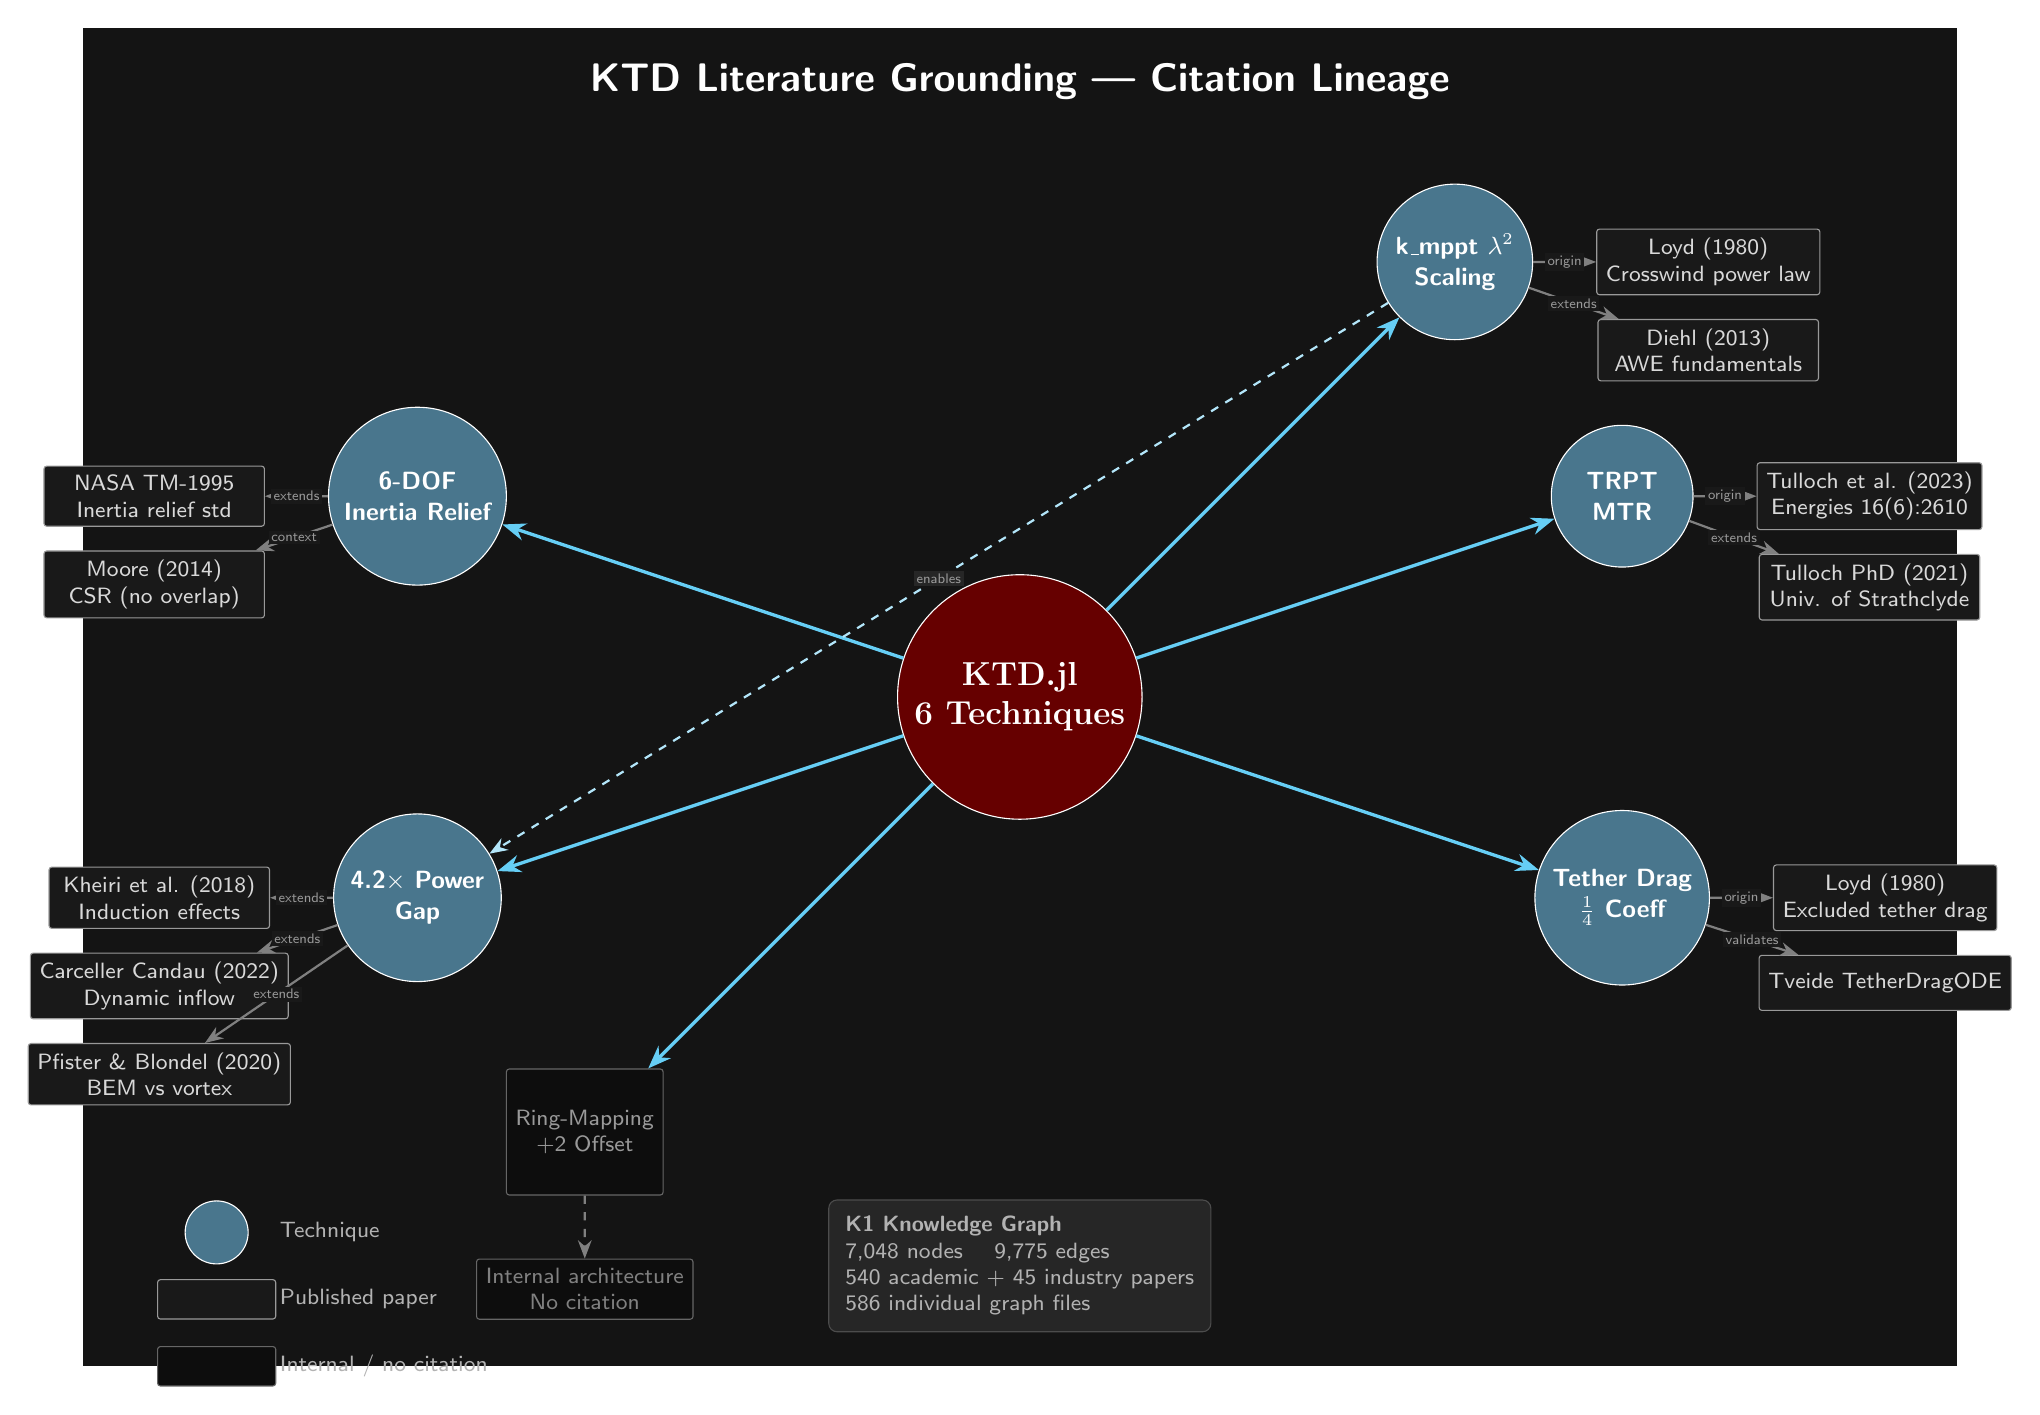
\begin{tikzpicture}[scale=0.85,
    technique/.style={circle, draw=white, fill=cyan!50!black, minimum size=18mm, font=\small\bfseries\sffamily, text=white, align=center},
    paper/.style={rectangle, draw=white!60!black, fill=white!10!black, minimum width=28mm, minimum height=7mm, font=\footnotesize\sffamily, text=white!85!black, align=center, rounded corners=1pt},
    internal/.style={rectangle, draw=white!40!black, fill=white!5!black, minimum width=22mm, minimum height=7mm, font=\footnotesize\sffamily, text=white!60!black, align=center, rounded corners=1pt},
    edge/.style={->, >=Stealth, white!50!black, line width=0.8pt},
    edgelabel/.style={font=\tiny\sffamily, text=white!60!black, fill=black!90, inner sep=1pt},
    title/.style={font=\Large\bfseries\sffamily, text=white},
]

\fill[black!92] (-14,-10) rectangle (14,10);

% === CENTRAL NODE ===
\node[technique, fill=red!40!black, minimum size=22mm, font=\large\bfseries] (ktd) at (0,0) {KTD.jl\\6 Techniques};

% === TECHNIQUE NODES (6 radiating outward) ===
% Right side
\node[technique] (t1) at (6.5,6.5) {k\_mppt $\lambda^2$\\Scaling};
\node[technique] (t2) at (9,3) {TRPT\\MTR};
\node[technique] (t3) at (9,-3) {Tether Drag\\$\frac14$ Coeff};
% Left side
\node[technique] (t4) at (-9,3) {6-DOF\\Inertia Relief};
\node[technique] (t5) at (-9,-3) {4.2$\times$ Power\\Gap};
\node[internal, minimum size=16mm] (t6) at (-6.5,-6.5) {Ring-Mapping\\+2 Offset};

% === KTD -> Technique edges ===
\foreach \t in {t1,t2,t3,t4,t5,t6} {
    \draw[edge, cyan!60, line width=1.2pt] (ktd) -- (\t);
}

% === PAPER NODES (connected to techniques) ===
% t1 (k_mppt)
\node[paper, right=0.8cm of t1] (p1a) {Loyd (1980)\\Crosswind power law};
\node[paper, below=0.3cm of p1a] (p1b) {Diehl (2013)\\AWE fundamentals};
\draw[edge] (t1) -- (p1a) node[edgelabel, midway] {origin};
\draw[edge] (t1) -- (p1b) node[edgelabel, midway] {extends};

% t2 (MTR)
\node[paper, right=0.8cm of t2] (p2a) {Tulloch et al. (2023)\\Energies 16(6):2610};
\node[paper, below=0.3cm of p2a] (p2b) {Tulloch PhD (2021)\\Univ. of Strathclyde};
\draw[edge] (t2) -- (p2a) node[edgelabel, midway] {origin};
\draw[edge] (t2) -- (p2b) node[edgelabel, midway] {extends};

% t3 (tether drag)
\node[paper, right=0.8cm of t3] (p3a) {Loyd (1980)\\Excluded tether drag};
\node[paper, below=0.3cm of p3a] (p3b) {Tveide TetherDragODE};
\draw[edge] (t3) -- (p3a) node[edgelabel, midway] {origin};
\draw[edge] (t3) -- (p3b) node[edgelabel, midway] {validates};

% t4 (6-DOF IR)
\node[paper, left=0.8cm of t4] (p4a) {NASA TM-1995\\Inertia relief std};
\node[paper, below=0.3cm of p4a] (p4b) {Moore (2014)\\CSR (no overlap)};
\draw[edge] (t4) -- (p4a) node[edgelabel, midway] {extends};
\draw[edge] (t4) -- (p4b) node[edgelabel, midway] {context};

% t5 (4.2x gap)
\node[paper, left=0.8cm of t5] (p5a) {Kheiri et al. (2018)\\Induction effects};
\node[paper, below=0.3cm of p5a] (p5b) {Carceller Candau (2022)\\Dynamic inflow};
\node[paper, below=0.3cm of p5b] (p5c) {Pfister \& Blondel (2020)\\BEM vs vortex};
\draw[edge] (t5) -- (p5a) node[edgelabel, midway] {extends};
\draw[edge] (t5) -- (p5b) node[edgelabel, midway] {extends};
\draw[edge] (t5) -- (p5c) node[edgelabel, midway] {extends};

% t6 (ring-mapping) --- internal, no papers
\node[internal, below=0.8cm of t6, font=\footnotesize\sffamily, text=white!50!black] (t6n) {Internal architecture\\No citation};
\draw[edge, dashed] (t6) -- (t6n);

% === INTER-TECHNIQUE EDGES (where they interact) ===
\draw[edge, cyan!30, dashed] (t1) -- (t5) node[edgelabel, midway, fill=black!85] {enables};

% === GRAPH STATS BOX ===
\node[draw=white!30!black, fill=black!85, rounded corners=3pt, inner sep=6pt, font=\footnotesize\sffamily, text=white!70!black, align=left] (stats) at (0,-8.5) {
    \textbf{K1 Knowledge Graph}\\
    7,048 nodes \quad 9,775 edges\\
    540 academic + 45 industry papers\\
    586 individual graph files
};

% === TITLE ===
\node[title] at (0,9.2) {KTD Literature Grounding --- Citation Lineage};

% === LEGEND ===
\node[technique, minimum size=8mm, font=\tiny] at (-12,-8) {};
\node[font=\footnotesize\sffamily, text=white!70!black, anchor=west] at (-11.2,-8) {Technique};
\node[paper, minimum width=15mm, minimum height=5mm, font=\tiny] at (-12,-9) {};
\node[font=\footnotesize\sffamily, text=white!70!black, anchor=west] at (-11.2,-9) {Published paper};
\node[internal, minimum width=15mm, minimum height=5mm, font=\tiny] at (-12,-10) {};
\node[font=\footnotesize\sffamily, text=white!70!black, anchor=west] at (-11.2,-10) {Internal / no citation};

\end{tikzpicture}
\end{document}
